\begin{solution}
\begin{enumerate}
\item {[5 points]} The general solution to
\[
-w''(x)=0
\]
is $w(x)=Ax+B$ where $A$ and $B$ are constants. Moreover, $w(0)=B$ and so $w(0)=0$ when $B=0$. Hence, $w(x)=Ax$ and so $w(1)=A$ and hence $w(1)=1$ when $A=1$. Consequently,
\[
w(x)=x.
\]
\\
\item {[5 points]} We can compute that $u(x,t)=w(x)+\hat{u}(x,t)$ will be such that
\[
u(x,0)=w(x)+\hat{u}(x,0)=x+\hat{u}_0(x)
\]
and so since
\[
u(x,0)=x^3
\]
we can conclude that
\[
\hat{u}_0(x)=x^3-x.
\]
\\
\item {[5 points]} Substituting the expressions for $\hat{u}(x,t)$ and $f(x)$ into the partial differential equation yields
\[
\sum_{n=1}^\infty a'_n(t) \psi_n (x)-\sum_{n=1}^\infty a_n(t) \left(-\left(L\psi_n\right) (x)\right)=\sum_{n=1}^\infty b_n \psi_n (x)
\]
and hence
\[
\sum_{n=1}^\infty \left(a'_n(t)+\lambda_na_n(t)\right)\psi_n (x)=\sum_{n=1}^\infty b_n \psi_n (x).
\]
We can then say that
\[
\sum_{n=1}^\infty \left(a'_n(t)+\lambda_na_n(t)\right)\int_0^1\psi_n (x)\psi_m (x)\,dx=\sum_{n=1}^\infty b_n \int_0^1\psi_n (x)\psi_m (x)\,dx
\]
for $m=1,2,\ldots$, from which it follows that
\[
a_m'(t)+\lambda_m a_m(t)=b_m
\]
for $m=1,2,\ldots$, since
\[
\int_0^1\psi_n (x)\psi_m (x)\,dx = \left\{\begin{array}{ll} 1 & \mbox{if }m=n, \\ 0 & \mbox{otherwise,} \end{array}\right.
\]
for $m,n=1,2,\ldots$. Now, for $n=1,2,\ldots$,
\begin{eqnarray*}
b_n&=&\int_0^1f(x)\psi_n(x)\,dx
\\
&=&\sqrt{2}\int_0^1 f(x)\sin(n\pi x)\,dx
\\
&=& \sqrt{2}\left(\int_0^{1/2} f(x)\sin(n\pi x)\,dx+\int_{1/2}^1 f(x)\sin(n\pi x)\,dx\right)
\\
&=& 2\sqrt{2}\left(\int_0^{1/2} x\sin(n\pi x)\,dx+\int_{1/2}^1 (1-x)\sin(n\pi x)\,dx\right)
\\
&=&2\sqrt{2}\left(\left[-{1 \over n\pi}x\cos(n\pi x)\right]_0^{1/2}+{1 \over n\pi}\int_0^{1/2} \cos(n\pi x)\,dx+\left[-{1 \over n\pi}(1-x)\cos(n\pi x)\right]_{1/2}^1-{1 \over n\pi}\int_{1/2}^1 \cos(n\pi x)\,dx\right)
\\
&=&2\sqrt{2}\left(-{1 \over 2n\pi}\cos\left({n\pi \over 2}\right)+{1 \over n\pi}\int_0^{1/2} \cos(n\pi x)\,dx+{1 \over 2n\pi}\cos\left({n\pi \over 2}\right)-{1 \over n\pi}\int_{1/2}^1 \cos(n\pi x)\,dx\right)
\\
&=&\frac{2\sqrt{2}}{n\pi}\left(\int_0^{1/2} \cos(n\pi x)\,dx-\int_{1/2}^1 \cos(n\pi x)\,dx\right)
\\
&=&\frac{2\sqrt{2}}{n\pi}\left(\left[{1 \over n\pi}\sin(n\pi x)\right]_0^{1/2}-\left[{1 \over n\pi}\sin(n\pi x)\right]_{1/2}^1\right)
\\
&=&\frac{2\sqrt{2}}{n\pi}\left({1 \over n\pi}\sin\left(\frac{n\pi}{2}\right)+{1 \over n\pi}\sin\left(\frac{n\pi}{2}\right)\right)
\\
&=&\frac{4\sqrt{2}}{n^2\pi^2}\sin\left(\frac{n\pi}{2}\right).
\end{eqnarray*}
Hence, for $n=1,2,\ldots$,
\[
a_n'(t)+n^2\pi^2 a_n(t)=\frac{4\sqrt{2}}{n^2\pi^2}\sin\left(\frac{n\pi}{2}\right).
\]

Also,
\[
\hat{u}(x,0)=x^3-x
\]
means that
\[
\sum_{n=1}^\infty a_n(0) \psi_n (x)=x^3-x
\]
and so
\[
\sum_{n=1}^\infty a_n(0) \int_0^1\psi_n (x)\psi_m (x)\,dx=\int_0^1\left(x^3-x\right)\psi_m (x)\,dx
\]
for $m=1,2,\ldots$, from which it follows that
\[
a_m(0)=\int_0^1\left(x^3-x\right)\psi_m (x)\,dx
\]
for $m=1,2,\ldots$, since
\[
\int_0^1\psi_n (x)\psi_m (x)\,dx = \left\{\begin{array}{ll} 1 & \mbox{if }m=n, \\ 0 & \mbox{otherwise,} \end{array}\right.
\]
for $m,n=1,2,\ldots$. Now, for $n=1,2,\ldots$,
\begin{eqnarray*}
\int_0^1\left(x^3-x\right)\psi_n(x)\,dx&=& \sqrt{2}\int_0^1 \left(x^3-x\right)\sin(n\pi x)\,dx
\\
&=&\sqrt{2}\left(\left[-{1 \over n\pi}\left(x^3-x\right)\cos(n\pi x)\right]_0^1+{1 \over n\pi}\int_0^1 \left(3x^2-1\right)\cos(n\pi x)\,dx\right)
\\
&=&{\sqrt{2} \over n\pi}\int_0^1 \left(3x^2-1\right)\cos(n\pi x)\,dx
\\
&=&{\sqrt{2} \over n\pi}\left(\left[{1 \over n\pi}\left(3x^2-1\right)\sin(n\pi x)\right]_0^1-{6 \over n\pi}\int_0^1 x\sin(n\pi x)\,dx\right)
\\
&=&-{6\sqrt{2} \over n^2\pi^2}\int_0^1 x\sin(n\pi x)\,dx
\\
&=&-{6\sqrt{2} \over n^2\pi^2}\left(\left[-{1 \over n\pi}x\cos(n\pi x)\right]_0^1+{1 \over n\pi}\int_0^1 \cos(n\pi x)\,dx\right)
\\
&=&-{6\sqrt{2} \over n^2\pi^2}\left(-{1 \over n\pi}\cos(n\pi)+{1 \over n\pi}\left[{1 \over n\pi} \sin(n\pi x)\right]_0^1\right)
\\
&=&{6\sqrt{2} \over n^3\pi^3}\cos(n\pi).
\end{eqnarray*}
Hence, for $n=1,2,\ldots$,
\[
a_n(0)={6\sqrt{2} \over n^3\pi^3}\cos(n\pi).
\]

Therefore, for $n=1,2,\ldots$, $a_n(t)$ is the solution to the differential equation
\[
a_n'(t)+n^2\pi^2 a_n(t)=\frac{4\sqrt{2}}{n^2\pi^2}\sin\left(\frac{n\pi}{2}\right)
\]
with initial condition
\[
a_n(0)={6\sqrt{2} \over n^3\pi^3}\cos(n\pi).
\]
\\
\item {[4 points]} For $n=1,2,\ldots$,
\begin{eqnarray*}
a_n(t)&=&{6\sqrt{2} \over n^3\pi^3}\cos(n\pi) e^{-n^2\pi^2t}+\int_0^te^{n^2\pi^2\left(s-t\right)}b_n\,ds
\\
&=&{6\sqrt{2} \over n^3\pi^3}\cos(n\pi) e^{-n^2\pi^2t}+\frac{4\sqrt{2}}{n^2\pi^2}\sin\left(\frac{n\pi}{2}\right)\int_0^te^{n^2\pi^2\left(s-t\right)}\,ds
\\
&=&{6\sqrt{2} \over n^3\pi^3}\cos(n\pi) e^{-n^2\pi^2t}+\frac{4\sqrt{2}}{n^2\pi^2}\sin\left(\frac{n\pi}{2}\right)\left[\frac{1}{n^2\pi^2}e^{n^2\pi^2\left(s-t\right)}\right]_{s=0}^{s=t}
\\
&=&{6\sqrt{2} \over n^3\pi^3}\cos(n\pi) e^{-n^2\pi^2t}+\frac{4\sqrt{2}}{n^2\pi^2}\sin\left(\frac{n\pi}{2}\right)\left(\frac{1}{n^2\pi^2}-\frac{1}{n^2\pi^2}e^{-n^2\pi^2t}\right)
\\
&=&{6\sqrt{2} \over n^3\pi^3}\cos(n\pi) e^{-n^2\pi^2t}+\frac{4\sqrt{2}}{n^4\pi^4}\sin\left(\frac{n\pi}{2}\right)\left(1-e^{-n^2\pi^2t}\right)
\\
&=&{2\sqrt{2} \over n^3\pi^3}\left(3\cos(n\pi) e^{-n^2\pi^2t}+\frac{2}{n\pi}\sin\left(\frac{n\pi}{2}\right)\left(1-e^{-n^2\pi^2t}\right)\right)
\\
&=&{2\sqrt{2} \over n^3\pi^3}\left(\frac{2}{n\pi}\sin\left(\frac{n\pi}{2}\right)+\left(3\cos(n\pi)-\frac{2}{n\pi}\sin\left(\frac{n\pi}{2}\right)\right) e^{-n^2\pi^2t}\right).
\end{eqnarray*}
\\
\item {[3 points]} We can write
\begin{eqnarray*}
u(x,t) &=& w(x)+\hat{u}(x,t)
\\
&=& x+\sum_{n=1}^\infty a_n(t) \psi_n(x)
\\
&=& x+\sum_{n=1}^\infty {2\sqrt{2} \over n^3\pi^3}\left(\frac{2}{n\pi}\sin\left(\frac{n\pi}{2}\right)+\left(3\cos(n\pi)-\frac{2}{n\pi}\sin\left(\frac{n\pi}{2}\right)\right) e^{-n^2\pi^2t}\right) \psi_n(x)
\\
&=& x+\sum_{n=1}^\infty {4 \over n^3\pi^3}\left(\frac{2}{n\pi}\sin\left(\frac{n\pi}{2}\right)+\left(3\cos(n\pi)-\frac{2}{n\pi}\sin\left(\frac{n\pi}{2}\right)\right)e^{-n^2\pi^2t}\right)\sin(n\pi x).
\end{eqnarray*}
\\
\item {[3 points]} The requested plot is below.

\begin{center}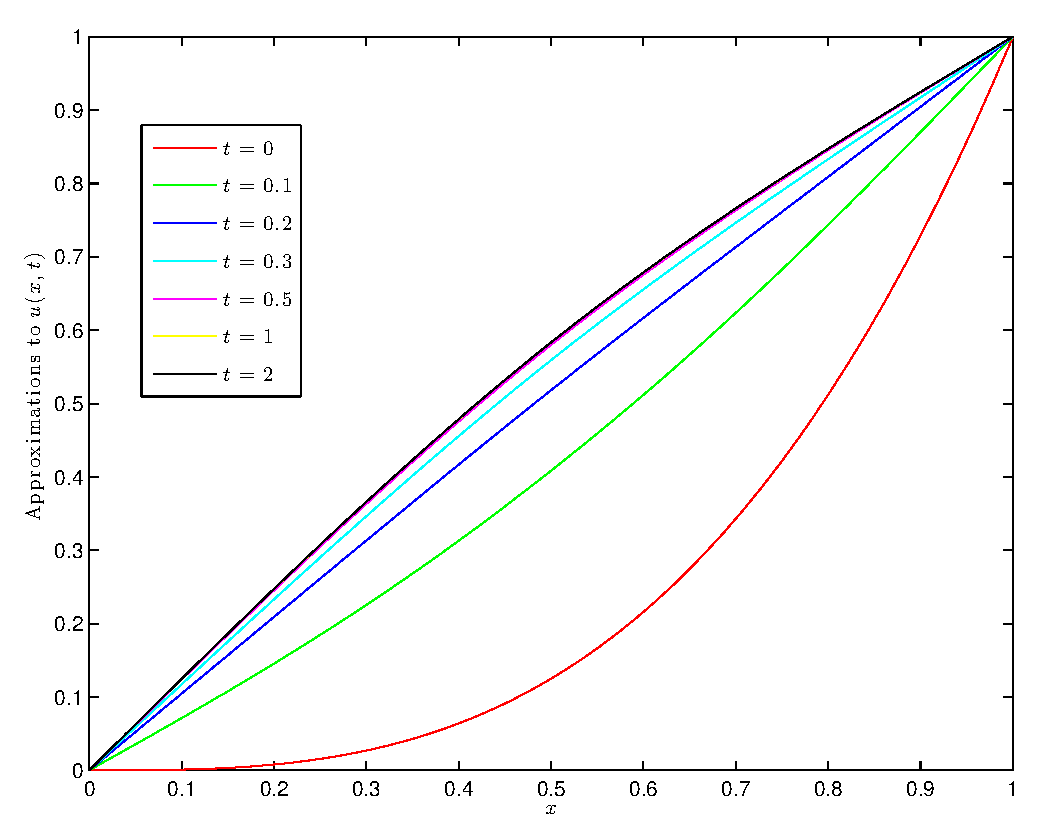
\includegraphics[scale=0.7]{hw39f.eps}\end{center}

The above plot was produced using the following MATLAB code.

\lstinputlisting{HW39f.m}

\end{enumerate}
\end{solution}